
\documentclass[border=8pt, multi, tikz]{standalone} 
\usepackage{import}
\subimport{../layers/}{init}
\usetikzlibrary{positioning}
\usetikzlibrary{3d} %for including external image 

\def\ConvColor{rgb:magenta,5;black,7}
\def\SoftmaxColor{rgb:yellow,6;red,6;white,3}
\def\PoolColor{rgb:red,1;black,0.3}
\def\UnpoolColor{rgb:blue,2;green,1;black,0.3}
\def\FcColor{rgb:blue,5;red,2.5;white,5}
\def\FcReluColor{rgb:blue,5;red,5;white,4}
\def\ConvReluColor{rgb:magenta,5;black,7}   
\def\ConcatColor{rgb:green,5;red,2;white,3}
\def\BERT{rgb:yellow,10;red,3;white,3}

 

\newcommand{\copymidarrow}{\tikz \draw[-Stealth,line width=0.8mm,draw={rgb:blue,4;red,1;green,1;black,3}] (-0.3,0) -- ++(0.3,0);}

\begin{document}
\begin{tikzpicture}
\tikzstyle{connection}=[ultra thick,every node/.style={sloped,allow upside down},draw=\edgecolor,opacity=0.7]
\tikzstyle{copyconnection}=[ultra thick,every node/.style={sloped,allow upside down},draw={rgb:blue,4;red,1;green,1;black,3},opacity=0.7]


%====================================================================================
\pic[shift={(-1.2,2.2,-1)}] at (-8,4,0) {RightBandedBox={name=News,caption=,%
        zlabel=News,fill=\BERT,bandfill=\BERT,%
        height=0,width={0},depth=9}};

\pic[shift={(-2,1.7,-2)}] at (-8,3,10) {RightBandedBox={name=Comments,caption=,%
        zlabel=Comments,fill=\BERT,bandfill=\BERT,%
        height=0,width={0},depth=15}};  
        
\pic[shift={(0,2.5,2)}] at (-5,3,28) {RightBandedBox={name=Tweet,caption=,%
        zlabel=Tweet,fill=\BERT,bandfill=\BERT,%
        height=0,width={0},depth=10}};

%====================================================================================

%\node[canvas is zy plane at x=0] (temp) at (-3,2,0) {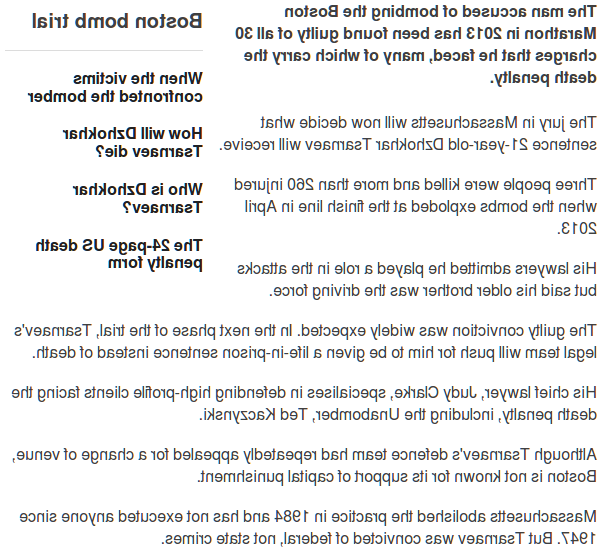
\includegraphics[scale=0.25]{news}};

%\node[canvas is zy plane at x=0] (temp) at (0,3,28) {
\includegraphics[scale=0.35]{tweet}};

%\node[canvas is zy plane at x=0] (temp) at (-3,2,10) {
\includegraphics[scale=0.35]{comments}};

\node[canvas is zy plane at x=0] (temp) at (-8,4,0) {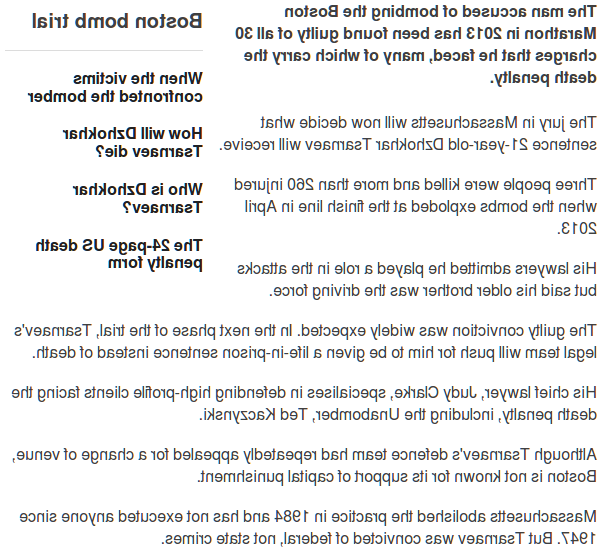
\includegraphics[scale=0.25]{news}};

\node[canvas is zy plane at x=0] (temp) at (-5,3,28) {
\includegraphics[scale=0.35]{tweet}};

\node[canvas is zy plane at x=0] (temp) at (-8,3,10) {
\includegraphics[scale=0.35]{comments}};


% Bert News
\pic[shift={(0,0,0)}] at (-4,1,-1) {RightBandedBox={name=bertN,caption=Encoder,%
        xlabel={{"."}},zlabel=512,fill=\BERT,bandfill=\BERT,%
        height=7,width={7},depth=40}};

% Input News
\pic[shift={(0,0,0)}] at (0,0,0) {RightBandedBox={name=inN1,caption=Input News,%
        xlabel={{"1"}}, zlabel=512,fill=\SoftmaxColor,bandfill=\SoftmaxColor,%
        height=2,width={2},depth=40}};

% News conv1
\pic[shift={(1,0,0)}] at (inN1-east) {RightBandedBox={name=convN1,caption=Conv1N,%
        xlabel={{"1 1 1 1 1"}},zlabel=508,fill=\ConvColor,bandfill=\ConvReluColor,%
        height=2,width={2,2,2,2,2},depth=30}};
        

\iffalse
% News Flatten 
\pic[shift={(1,0,0)}] at (convN1-east) {RightBandedBox={name=flatN,caption=Fla,%
        zlabel=2540,fill=\FcColor,bandfill=\FcReluColor,%
        height=2,width=2,depth=80}};
\fi

% Bert Tweet
\pic[shift={(0,0,0)}] at (-4,1,12) {RightBandedBox={name=bertT,caption=Encoder,%
        xlabel={{"."}},zlabel=512,fill=\BERT,bandfill=\BERT,%
        height=7,width={7},depth=40}};
        
% Input Tweet       
\pic[shift={(-10,-10,0)}] at (0,0,0) {RightBandedBox={name=inT1,caption=Input Tweet,%
        xlabel={{"1"}},zlabel=512,fill=\SoftmaxColor,bandfill=\SoftmaxColor,%
        height=2,width={2},depth=40}};

% Tweet conv1
\pic[shift={(1,0,0)}] at (inT1-east) {RightBandedBox={name=convT1,caption=Conv1T,%
        xlabel={{"1 1 1 1 1"}},zlabel=510,fill=\ConvColor,bandfill=\ConvReluColor,%
        height=2,width={2,2,2,2,2},depth=30}};
        
        
\iffalse
% Tweet Flatten        
\pic[shift={(1,0,0)}] at (convT1-east) {RightBandedBox={name=flatT,caption=Fla,%
        zlabel=2550,fill=\FcColor,bandfill=\FcReluColor,%
        height=2,width=2,depth=80}};
\fi

% Bert Comments
\pic[shift={(0,0,0)}] at (-4,1,24) {RightBandedBox={name=bertC,caption=Encoder,%
        xlabel={{"."}},zlabel=512,fill=\BERT,bandfill=\BERT,%
        height=7,width={7},depth=40}};

% Input Comments
\pic[shift={(-1,0,12.5)}] at (0,0,0) {RightBandedBox={name=inC1,caption=Input Comments,%
        xlabel={{"1"}},zlabel=512,fill=\SoftmaxColor,bandfill=\SoftmaxColor,%
        height=2,width={2},depth=40}};

% Comments conv1
\pic[shift={(1,0,0)}] at (inC1-east) {RightBandedBox={name=convC1,caption=Conv1C,%
        xlabel={{"1 1 1 1 1"}},zlabel=510,fill=\ConvColor,bandfill=\ConvReluColor,%
        height=2,width={2,2,2,2,2},depth=30}};

% Concatenation
\pic[shift={(-1,-4, 8)}] at (convN1-east) {RightBandedBox={name=conc,caption=Conc,%
        zlabel=7640,fill=\UnpoolColor,bandfill=\UnpoolColor,%
        height=2,width=2,depth=100}};
        
% First Dense
\pic[shift={(1.5,0,0)}] at (conc-east) {RightBandedBox={name=dense1,caption=FC1 / Pooling,%
        zlabel=198,fill=\ConcatColor,bandfill=\ConcatColor,%
        height=2,width=2,depth=50}};

% Average Pooling        
\pic[shift={(0,0,0)}] at (dense1-east) {Box={name=avgPool,%
       fill=\PoolColor,opacity=0.5,height=2,width=0.3,depth=45}};

% First Conv        
\pic[shift={(1,0,0)}] at (avgPool-east) {RightBandedBox={name=conv1,caption=Conv2,%
        xlabel={{"1 1 1 1 1"}}, zlabel=196,fill=\ConvColor,bandfill=\ConvReluColor,%
        height=2,width={2,2,2,2,2},depth=45}};

% Second Conv
\pic[shift={(1,0,0)}] at (conv1-east) {RightBandedBox={name=conv2,caption=Conv3,%
        xlabel={{"1 1 1"}}, zlabel=195,fill=\ConvColor,bandfill=\ConvReluColor,%
        height=2,width={2,2,2},depth=40}};
\iffalse
% First Flatten   
\pic[shift={(3,0,0)}] at (conv2-east) {RightBandedBox={name=flat1,caption=Fla,%
        zlabel=585,fill=\FcColor,bandfill=\FcReluColor,%
        height=2,width=2,depth=60}};
\fi
% Second Dense
\pic[shift={(1,0,0)}] at (conv2-east) {RightBandedBox={name=dense2,caption=FC2,%
        zlabel=150,fill=\ConcatColor,bandfill=\ConcatColor,%
        height=2,width=2,depth=35}};
        
% Third Conv
\pic[shift={(1,0,0)}] at (dense2-east) {RightBandedBox={name=conv3,caption=Conv4,%
        xlabel={{"1 1 1 1 1"}}, zlabel=149,fill=\ConvColor,bandfill=\ConvReluColor,%
        height=2,width={2,2,2,2,2},depth=30}};

% Third Dense
\pic[shift={(1,0,0)}] at (conv3-east) {RightBandedBox={name=dense3,caption=FC3,%
        zlabel=70,fill=\ConcatColor,bandfill=\ConcatColor,%
        height=2,width=2,depth=25}};  
        
% Fourth Dense
\pic[shift={(1,0,0)}] at (dense3-east) {RightBandedBox={name=dense4,caption=FC4-ReLu,%
        zlabel=3,fill=\ConcatColor,bandfill=\ConcatColor,%
        height=2,width=2,depth=20}}; 
        
% Draw Connections 

\draw [connection]  (bertN-east)        -- node {\midarrow} (inN1-west);
\draw [connection]  (bertT-east)        -- node {\midarrow} (inC1-west);
\draw [connection]  (bertC-east)        -- node {\midarrow} (inT1-west);

\draw [connection]  (inT1-east)        -- node {\midarrow} (convT1-west);
\draw [connection]  (inN1-east)        -- node {\midarrow} (convN1-west);
\draw [connection]  (inC1-east)        -- node {\midarrow} (convC1-west);

\draw[densely dashed]
        
    (convT1-nearsoutheast) coordinate(a) -- (conc-nearsoutheast)
    (convT1-farsoutheast) coordinate(b) -- (conc-east)
    
    (convN1-nearsoutheast) coordinate(c) -- (conc-east)
    (convN1-farsoutheast) coordinate(d) -- (conc-farsoutheast)
    
    (convC1-nearsoutheast) coordinate(c) -- (conc-east)
    (convC1-farsoutheast) coordinate(d) -- (conc-east)
    
    
%    (a)--(b)--(c)--(d)
    ;

\draw [connection]  (conc-east)        -- node {\midarrow} (dense1-west);
\draw [connection]  (dense1-east)        -- node {\midarrow} (conv1-west);
\draw [connection]  (conv1-east)        -- node {\midarrow} (conv2-west);
\draw [connection]  (conv2-east)        -- node {\midarrow} (dense2-west);
\draw [connection]  (dense2-east)        -- node {\midarrow} (conv3-west);
\draw [connection]  (conv3-east)       -- node {\midarrow} (dense3-west);
\draw [connection]  (dense3-east)       -- node {\midarrow} (dense4-west);

\end{tikzpicture}
\end{document}
